\documentclass[12pt,letterpaper]{article}
\usepackage{pdfpages}
\usepackage{fancyhdr}
\usepackage[colorlinks=true, urlcolor=blue, linkcolor=blue]{hyperref}
\usepackage{graphicx}
\usepackage[top=1.4in, left=0.5in, right=0.5in, bottom=0.8in]{geometry}
\usepackage[T1]{fontenc}
\usepackage{helvet}
\pagestyle{fancy}
\renewcommand{\headrulewidth}{0pt}
\renewcommand{\footrulewidth}{0pt}
\setlength{\parindent}{0em}
\setlength{\parskip}{1em}


\fancyfoot[C]{\setlength{\unitlength}{1in}\begin{picture}(5,0)\put(-1.8,-1){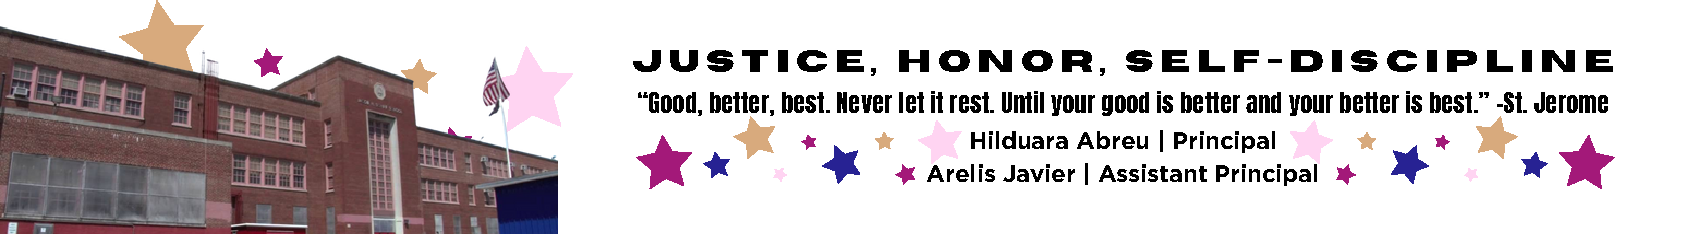
\includegraphics[width=8.8in,height=1.3in]{logo-1}}\end{picture}}
\fancyhead[C]{\setlength{\unitlength}{1in}\begin{picture}(5,0)\put(-1.9,-1){
\includegraphics[width=8.9in,height=1.3in]{logo-2}}\end{picture}}

\pagenumbering{gobble}
\addtolength{\evensidemargin}{-2in}
\addtolength{\topmargin}{-0.5in}
\addtolength{\textwidth}{0in}
%%%%%%%%%%%%%%%%%%%%%%%%%%%%%%%%%%%%%%%%%%%%%%%%%%%%%%%%%%%%%%%%%%

\begin{document}
\vspace*{0.5in}
Date: \href{https://www.ps192.org/apps/bbmessages/show_bbm.jsp?REC_ID=139439}{September 14, 2023} 

\textbf{Asunto: Año Escolar 2023-24 | PS 192 Procedimientos de Seguridad y para Visitantes}

Queridos padres y guardianes,

Nos complace presentar las pautas y procedimientos de nuestra estimada institución, Jacob H. Schiff/P.S. 192. Estas pautas y procedimientos han sido diseñados meticulosamente para priorizar la seguridad de todas las personas (nuestros valiosos estudiantes, personal dedicado y visitantes respetados) al tiempo que fomentan un ambiente acogedor e inclusivo. Agradecemos sinceramente su cooperación para cumplir con estos protocolos esenciales.
\begin{itemize}
	\item Registro de visitantes:
		\begin{itemize}
		\item A su llegada: Todos los visitantes, incluidos padres, tutores,
Se ruega a los voluntarios, contratistas y estimados invitados que Ingrese a las instalaciones de la escuela por la entrada principal y diríjase a la mostrador del agente de seguridad para registrarse.
		\item Cálida bienvenida: nuestro agente de seguridad escolar o personal escolar designado Dará una calurosa bienvenida a todos los visitantes, pregunte sobre el propósito de su visite y solicite una identificación con fotografía válida.
		\item Identificación: Para garantizar la seguridad, los visitantes deben presentar una identificación válida.
forma de identificación, como una licencia de conducir, emitida por el gobierno
DNI, pasaporte extranjero o estadounidense, o cédula de identidad consular.
Posteriormente se entregará a los visitantes una pegatina identificativa, que
deben exhibirse de manera destacada durante su visita. La seguridad escolar
El agente le ayudará a emitir la etiqueta de identificación.
		\item Notificación de Asistencia: Una vez que el Agente de Seguridad 
		Escolar o El personal escolar designado completa el proceso de 
		inscripción, notificar al coordinador de padres llamando al X1190. Esto facilitará asistencia adicional para el visitante, ya sea esperando en el vestíbulo o en el sala.
		\item Protocolo de salida: Se ruega a los visitantes que firmen su 
		salida con el Agente de Seguridad Escolar o el personal escolar 
		designado al salir de la edificio. Se deberá devolver la pegatina de 
		identificación; el principal La entrada es el punto de salida 
		recomendado.
		\end{itemize}
	\item Asistencia lingüística:
		\begin{itemize}
		\item Cuando un visitante no se comunica en inglés, nuestro Agente de Seguridad Escolar (SSA) o miembro designado del personal escolar intentará identificar el idioma del visitante. Se utilizará un cartel en varios idiomas exhibido en el mostrador de seguridad para la identificación del idioma. Una vez que se determine el idioma, el visitante será dirigido al coordinador de padres para obtener más ayuda. En los casos en los que necesitemos personal que domine el idioma del
\pagebreak
\vspace*{1.5cm}
visitante en el sitio, el coordinador de padres contratará a la Unidad de interpretación telefónica del DOE para concertar un intérprete a pedido.
		\end{itemize}
	\item Citas:
		\begin{itemize}
		\item Política de puertas abiertas: todos los martes de 2:20 a 3:00 p. m., TODOS los miembros del personal están disponibles para reuniones con padres/cuidadores.
		\item Visitas programadas: Recomendamos que se programen visitas que no sean de emergencia siempre que sea posible para garantizar que los miembros del personal estén disponibles para reunirse con los visitantes y minimizar la interrupción del tiempo de instrucción. Los visitantes y el personal pueden programar citas a través de varios canales, incluido Classdojo, el correo electrónico directo del personal, el sitio web de nuestra escuela o comunicarse con el coordinador de padres.
		\item Llegada de visitantes: Al llegar a una cita programada, se solicita a los visitantes que sigan el mismo proceso de entrada y registro descrito anteriormente.
		\end{itemize}
	\item Escolta y Supervisión:
		\begin{itemize}
		\item Escolta de visitantes: para mayor seguridad, un miembro del personal designado acompañará a los visitantes hacia y desde su destino previsto dentro de las instalaciones de la escuela, incluidos los salones de clases, las oficinas, la biblioteca, el gimnasio y otros espacios compartidos.
		\item Contacto supervisado: Los visitantes deben interactuar con los estudiantes solo si están expresamente autorizados por la administración de la escuela o como parte de un programa o evento previamente aprobado.
		\end{itemize}
	\item Confidencialidad y Privacidad:
		\begin{itemize}
		\item Medios y Privacidad: Para mantener la privacidad y confidencialidad de nuestros estudiantes y miembros del personal, se solicita a los visitantes que no tomen fotografías ni graben videos mientras se encuentren en las instalaciones de la escuela.
		\item Respeto a la privacidad: cualquier información personal u observación realizada durante la visita no debe compartirse sin el consentimiento o autorización correspondiente del Departamento de Educación de la Ciudad de Nueva York.
		\end{itemize}
	\item Simulacros de seguridad:
		\begin{itemize}
		\item A lo largo del año académico, llevamos a cabo simulacros de seguridad para garantizar que los estudiantes y el personal estén bien preparados para responder eficazmente en caso de emergencias. Estos simulacros son esenciales para la seguridad de nuestra comunidad escolar e incluyen:
			\begin{itemize}
			\item 12 simulacros de incendio: realizados quincenalmente de septiembre al 31 de diciembre de 2023 y posteriormente mensualmente.
			\pagebreak
\vspace*{1.5cm}
			\item 4 simulacros de encierro: realizados cada dos meses.
			\item 2 Simulacros de Emergencia en Autobús: Realizados al inicio del año escolar e inicio del segundo semestre (febrero 2024).
			\end{itemize}
		\end{itemize}
\end{itemize}

Al seguir fielmente estas pautas y procedimientos para visitantes, contribuimos colectivamente a la seguridad y el bienestar de nuestra estimada comunidad escolar. Si tiene alguna pregunta o necesita más aclaraciones, no dude en contactarnos o comunicarse con la Sra. Rijo al 646-745-0150 o al 212-775-9560 X1190. Su compromiso y apoyo inquebrantables son fundamentales para mantener un entorno de aprendizaje positivo y seguro. También hay asistencia adicional disponible a través de nuestro sitio web o WhatsApp.

Una vez más, extendemos nuestro más sincero agradecimiento por su cooperación y dedicación a nuestra misión compartida.

En unidad,


\includegraphics[width=0.2\textwidth]{hil_signature}

\textbf{Hilduara Abreu}

\textbf{Principal}

\textit{La escuela donde el aprendizaje es divertido!}

\url{www.ps192.org}

\end{document}
